\chapter{ダウン・サンプリング}
    \section{ダウン・サンプリングされた信号のDTFT}
        \newcommand{\xd}{x_\text{d}}
        \newcommand{\yd}{y_\text{d}}
        \newcommand{\Xd}{X_\text{d}}
        \newcommand{\Yd}{Y_\text{d}}
        \subsection{主張}
            記号を次のように定義する。
            \begin{itemize}
                \item $R\in\naturalNumbers,\;R\geq 2$ : ダウン・サンプリング・レート
                \item $\xd:\integers\to\complexNumbers$ : 離散時間信号
                \item $\Ts>0$ : $\xd$ のサンプル周期
                \item $\yd$ : $\xd$ を $1/R$ にダウン・サンプリングした離散時間信号。つまり $\yd(n) = \xd(nR)$ 。
                \item $\Xd$ : $\xd$ のDTFT
                \item $\Yd$ : $\yd$ のDTFT
            \end{itemize}
            このとき $\Yd$ は次式で表される。
            \[ \Yd(\omega) = \frac{1}{R}\sum_{n=-\floor{R/2}}^{\floor{R/2}} \integrate{-\pi/\Ts}{\pi/\Ts}{\Xd(\omega-\tilde{\omega})\delta\parens*{\tilde{\omega}-n\frac{2\pi}{R\Ts}}}{}{\tilde{\omega}} \]
            $\Yd$ は $\omega$ に関する $2\pi/(R\Ts)$ 周期関数となり、$\Yd$ の第1 Nyquist 領域は $S_{\text{N},Y} \coloneqq [-\pi/(R\Ts),-\pi/(R\Ts))$ となる。
            \par
            $\Xd$ の台のうち $\xd$ の第1 Nyquist 領域 $S_{\text{N},X} \coloneq [-\pi/\Ts, \pi/\Ts)$ にある部分を $S_X$ とする。
            エイリアシングが生じない必要十分条件は $S_X\subset S_{\text{N},X}$ である。
            ここで言うエイリアシングとは、$S_X$ を $2\pi/(R\Ts)$ の整数倍ずつ平行移動しながら無限に複製したものを考えたとき、複製された $S_X$ 同士に重なりが生じることを指す。
        \subsection{導出}
            \begin{align*}
                \Yd(\omega) &= \sum_{n=-\infty}^\infty \yd(n)\exp(-i\omega nR\Ts) = \sum_{n=-\infty}^\infty \xd(nR)\exp(-i\omega nR\Ts) \\
                &= \sum_{m=-\infty}^\infty u(m)\xd(m)\exp(-i\omega m\Ts) \quad \text{where} \quad u(m) \coloneqq \begin{cases}
                    1 & (m\in R\integers) \\
                    0 & (\text{otherwise})
                \end{cases} \\
                &= \DTFTwithArg{u\xd}{\omega} \\
                &= \frac{\Ts}{2\pi}\integrate{-\pi/\Ts}{\pi/\Ts}{\Xd(\omega-\tilde{\omega})U(\tilde{\omega})}{}{\tilde{\omega}} \quad \text{where} \quad U(\omega) \coloneqq \frac{2\pi}{R\Ts}\sum_{m=-\infty}^\infty\delta\parens*{\omega - n\frac{2\pi}{R\Ts}} \\
                &= \frac{1}{R} \integrate{-\pi/\Ts}{\pi/\Ts}{\Xd(\omega-\tilde{\omega})\sum_{n=-\infty}^{\infty}\delta\parens*{\tilde{\omega}-n\frac{2\pi}{R\Ts}}}{}{\tilde{\omega}} \tag{1}
            \end{align*}
            被積分関数の $\Xd$ とデルタ関数列を次の図に示す。
            \begin{figure}[H]
                \centering
                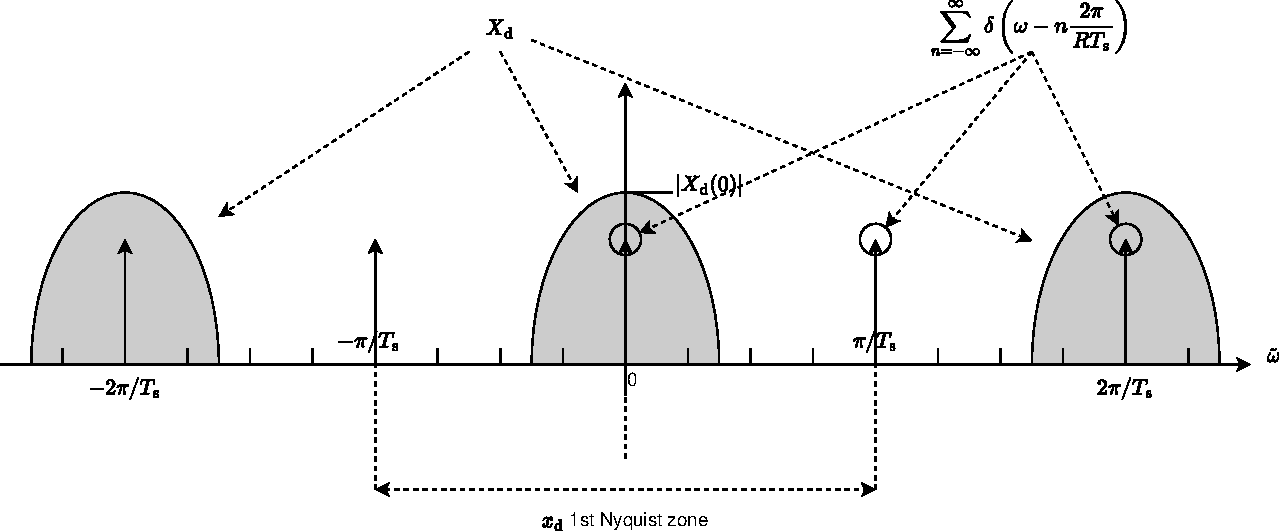
\includegraphics[keepaspectratio, scale=0.7]
                {\currfiledir/imgs/X_d_and_delta_impulse_series.pdf}
                \caption{$\Xd$ とデルタ関数列($R=2$)}
            \end{figure}
            $\Xd$ が $2\pi/\Ts$ 周期関数であること、式(1)の積分範囲が $[-\pi/\Ts,\pi/\Ts]$ であること、および $R$ が偶数の場合に積分範囲の両端点で生じる、デルタ関数の中心から左右半分と $\Xd$ との積の積分を考慮すると、式(1)は次式と等しいことが解る。
            \[ \frac{1}{R}\sum_{n=-\floor{R/2}}^{\floor{R/2}} \integrate{-\pi/\Ts}{\pi/\Ts}{\Xd(\omega-\tilde{\omega})\delta\parens*{\tilde{\omega}-n\frac{2\pi}{R\Ts}}}{}{\tilde{\omega}} \]
            また同時に、$\Yd$ が $\omega$ に関する $2\pi/(R\Ts)$ 周期関数であることも解る。
            \par
            エイリアシングが生じないことと $S_X \subset S_{N,\text{X}}$ が同値であることが解る。
            $\Yd$ を次の図に示す。
            \begin{figure}[H]
                \centering
                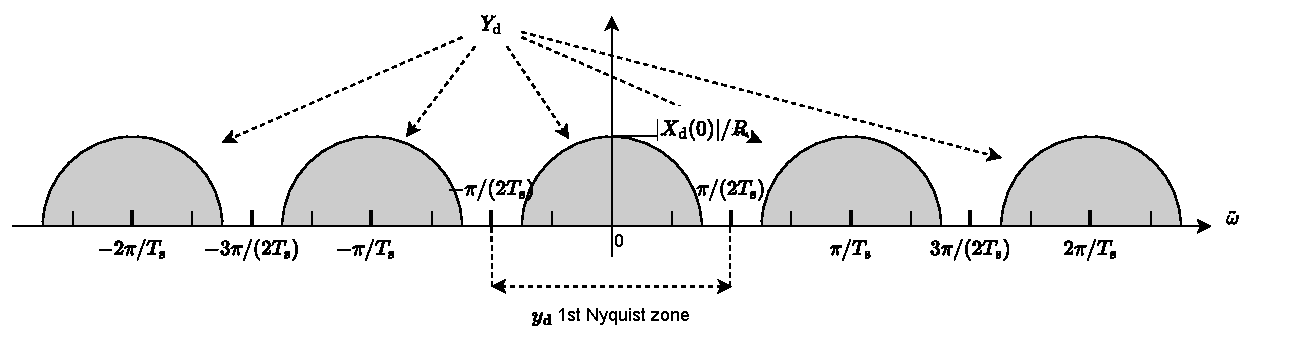
\includegraphics[keepaspectratio, scale=0.7]
                {\currfiledir/imgs/Yd.pdf}
                \caption{$\Yd$}
            \end{figure}
        \subsection{数値例}
            いくつかの数値例が下記の Mathematica ノートブックにある。
            \begin{itemize}
                \item \verb|DTFT_of_down-sampled_signal.nb|: $x(t) = A\exp(-t^2/(2\sigma^2))$
                \item \verb|DTFT_of_down-sampled_signal_example2.nb|: $x(t) = e^{-12.5 t^2}\cos(10\pi t)$
            \end{itemize}
